\section{Introduction}
\paragraph{Motivating example} Consider two hikers (Felix and Gabrielle) that each go on an hour-long hike round-trip from Nice. They each record their altitude. From both recordings, can be determine if they took the same route (in altitude at least)? If they did indeed take the same route, they can have different speeds at different parts of the hour. For instance, Felix may be quicker than Gabrielle when going uphill but tends to be slower when going downhill. This warps their altitude profile as a function of time: Felix seems to have climbed steeper ascents and Gabrielle to have descended steeeper descents.
\missingfigure{hiking example}
We model their profiles by two functions $f:[0,1] \to [0, \infty[$ and $g:[0, 1] \to [0, \infty[$. We can model the time-warp caused by their differences in speed by a \emph{reparametrization} of time, i.e. the existence of an increasing diffeomorphism on $[0,1]$, such that $g$ is equal to $f$ composed with the reparametrization. More formally, we would have $g = f \circ Q$ where $Q$ is the reparametrization. Our goal in this work is to develop a divergence $d$ that compares $f$ and $g$ with a divergence $d$ such that $d(f, g)=0$ if there exists $Q$ such that $g = f \circ Q$.

\paragraph{Time series alignment}
Time-series are ubiquitous in data analysis applications. Some common tasks include forecasting, classification, clustering. These tasks rely on pair-wise comparaisons of time series, whether as loss functions (for example for training a forecaster), for feature engineering or in a classifier or as the distance function in clustering.

Time-series cannot be compared as if they were vectors in Euclidean space. First, the length of the time-series can vary. Second, the points are not necessarily aligned in time: time warping, shifting, ... can be important to ignore in certain applications. In this work we focus on time warping, i.e. the transformation of time interval $[0,1]$ by a smooth reparametrization, i.e. an increasing diffeomorphism.


\paragraph{DTW family of divergences} Dynamic Time Warping (DTW) was introduced by \cite{missing} to compare time series and is the \emph{de facto} standard for comparing time series. Intuitively, Dynamic Time Warping finds a matching between the points in each time series, while respecting the order of the points. More precisely, the cost incurred by each matching is the euclidean distance between the points, the DTW distance between two time series in the sum of the costs. Formally, consider $\mathcal A_{n, m}$ the set of alignment matrices, i.e. binary matrices of size $n\times m$ such that $A_{1,1}=A_{n, m}=1$ and if $A_{i,j} = 1$ then exactly one of the following is true: $A_{i+1, j}=1$ or $A_{i, j+1}=1$ or $A_{i+1, j+1}=1$. Then DTW is defined by
\begin{equation}
    d_{DTW}((f_1, \ldots, f_n), (g_1, \ldots, g_m)) = \min_{A_\pi \in\mathcal A_{n, m}} \langle A_\pi, D(f, g)\rangle
\end{equation}
$\mathcal A_{n,m}$ is the set of alignments and has exponential cardinality in $n, m$, though DTW can be computed in $O(nm)$ time thanks to dynamic programming.

It is differentiable with respect to one of its inputs as soon as there is a unique solution to the matching (that does not make the DTW zero). Non-differentiability can happen in innocuous situations as illustrated in \cite{tavenar-dtw-diff}

Soft Dynamic Time Warping (sDTW) was proposed in \cite{sdtw} by replacing the $\min$ operator by a softened $\min^\gamma$ operator:
\begin{equation}
d_{DTW}^\gamma((f_1, \ldots, f_n), (g_1, \ldots, g_m)) = -\gamma \log \sum_{A \in \mathcal A_{n,m}}\exp\left(-\frac{\langle A, D(f, g)\rangle}{\gamma}\right)
\end{equation}
if $\gamma > 0$ and is equal to $d_{DTW}$ if $\gamma=0$.
Empirically, sDTW behaves similarly to DTW, has equivalent computational complexity, is differentiable, and works better than DTW-based DBA for averaging based methods like clustering.

\paragraph{Prior work}
Other approaches have been proposed: \cite{ref} applies an approximation of the Fréchet distance, \cite{ref} makes DTW more robust to shifts, \cite{ref} combines DTW with the Fréchet distance.

\todo[inline]{Add problem statement... so what?}
\paragraph{Approach \& Contributions}
DiffyTW is divergence between functions on $[0,1]$ representing time-series. It is provably invariant to subset of smooth reparametrizations. The set of transformations it is invariant to can be tuned. It can be robustly and efficiently used to compare time-series, by solving a quadratic program. DiffyTW is differentiable with respect to its input and can be integrated in wider machine learning workflows. We illustrate and study DiffyTW's behavior on time series empirically.

\paragraph{Notation} In this chapter, a time series is represented by a sample pattern $(t_i)_{1 \leq i \leq n}$ such that $0 \leq t_1 < \ldots < t_n \leq 1$ (not necessarily random) and values $(f_i)_{1\leq i\leq n}$ where $f_i \in\mathbb R^d$. $\mathcal H$ is a Hilbert space, generally the Reproducing Kernel Hilbert space of a kernel $K$. $\mathcal Q$ is a set of diffeomorphisms on $[0,1]$. Functions $f,g:[0,1] \to \mathcal X$, where $\mathcal X$ is a metric space, generally $\mathcal R^d$.

\section{DiffyTW}
\emph{In this section, we introduce \texttt{DiffyTW}, a dissimilarity between functions $[0,1] \to \mathcal X$ which is invariant to a chosen class of diffeomorphic reparametrizations of $[0,1]$.}

\subsection{Intuition}
Let $\mathcal Q$ be a set of increasing diffeomorphisms on $[0,1]$. Our goal is to concieve a divergence such that $d(f\circ Q, f) = 0$ for any $Q\in\mathcal Q$ and any $f:[0,1] \to \mathbb R^d$.

A key idea is to compare the integrals of $f\circ Q$ and $f$. Indeed, this allows one to apply the change of variable theorem:

\begin{equation}
\int_0^1 f\circ Q(x)Q^\prime(x)dx = \int_0^1 f(x)dx.
\end{equation}

Then,
%\begin{equation}
$q \mapsto \left\vert\int_0^1 f\circ Q(x)q(x) dx - \int_0^1 f(x)dx\right\vert$
%\end{equation}
is minimized by $q=Q^\prime$

However, $q=Q^\prime$ is not necessarily the only minimizer. Indeed, if $f:[0,1] \to \mathbb R$, then $q(x) = f(x) / f\circ Q(x)$ also minimizes this quantity.

To avoid these minimizers, consider two refinements: first, embed $f$ using an embedding map $\phi$ such that $\int \phi(f(x))dx$ is close to characterizing $f$ ; second, restrict the search space to the derivatives of reparametrizations.

\subsection{Definition of DiffyTW}

Let $\mathcal F$ be a space of functions $[0, 1] \to \mathbb R$. Let $\mathcal F_{0,1} \subset \mathcal F$ be a subset of $\mathcal F$ such that if $q\in\mathcal F_{0,1}$, $q\geq 0$ and $\int_0^1q(t)dt =1$. $\mathcal F_{0,1}$ defines the class of diffeormophic reparametrizations the divergence is invariant to through its derivatives. We denote $\mathcal Q$ the set of reparametrizations obtained by integrating the elements of $\mathcal F_{0,1}$, i.e.
\begin{equation}
    \mathcal Q = \left\lbrace Q: x\in[0,1] \mapsto \int_0^x q(x)dx ~\vert~ q \in \mathcal F_{0,1}\right\rbrace
\end{equation}

\begin{definition}[DiffyTW]\label{def:diffytw}
Let $d: \mathcal X^{[0,1]} \times \mathcal X^{[0,1]} \to \mathbb R^+$ be for any $f, g\in\mathcal X^{[0,1]}$,
\begin{equation}\label{eq:diffytw}
    d(f, g) = \min_{q \in \mathcal F_{0,1}}\left\Vert \int_0^1 \phi(f(x))q(x)dx - \int_0^1\phi(g(x))dx\right\Vert^2_\mathcal H.
\end{equation}
We call this divergence DiffyTW.
\end{definition}

Note that as soon as $f$ and $g$ and measurable, then $d$ is well defined. Indeed, since $\phi$ is bounded on $[0,1]$ and $q$ is integrable, the integrals are well-defined Bochner integrals and $d(f, g)$ is finite and well-defined.

\paragraph{Time-series alignment}
If $f$ and $g$ are two functions representing two time-series, DiffyTW aligns $f$ and $g$. Indeed, we can --applying the change of variable theorem -- rewrite \cref{eq:diffytw} as
\begin{equation}\label{eq:diffytw-Q}
    d(f, g) = \min_{Q \in \mathcal Q} \left\Vert \int_0^1 \phi(f \circ Q^{-1}(x))dx - \int_0^1\phi(g(x))dx\right\Vert^2_\mathcal H
\end{equation}

\noindent \Cref{eq:diffytw-Q} shows we that the minimizer of the optimization problem in \cref{eq:diffytw} is the derivative of the reparametrization that aligns $f$ with $g$ in terms of the embedding $f \mapsto \int \phi(f(x))dx$.

We adopt the following notation for convenience:
\begin{equation}\label{def:diffytw-delta}
\Delta(f , g) = \left\Vert \int_0^1 \phi(f(x))dx - \int_0^1\phi(g(x))dx\right\Vert^2_\mathcal H
\end{equation}

\begin{figure}[ht!]
\centering
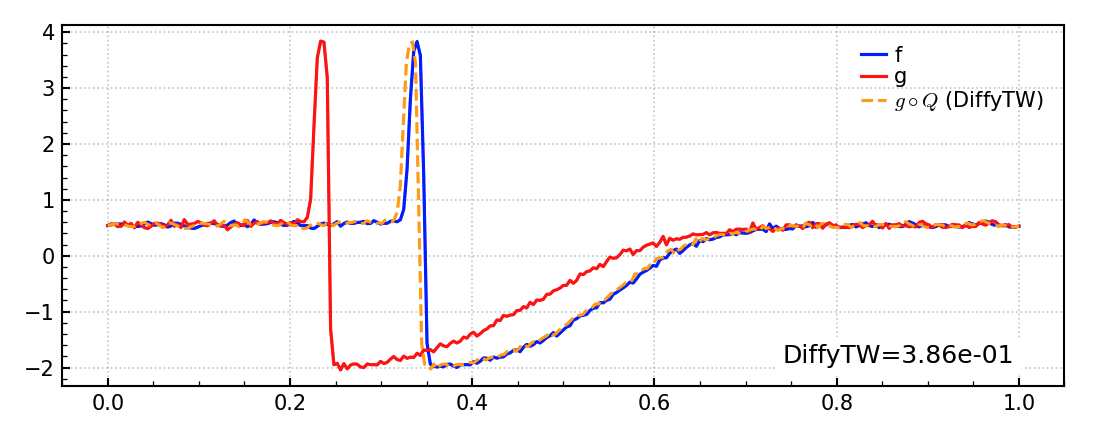
\includegraphics[width=0.8\textwidth]{ch3-diffytw/figures/diffytw-example.png}
\caption{Example of time-series alignment.}
\end{figure}

\subsection{Invariance to time-warping}
DiffyTW was designed to be equal to zero when comparing functions that are diffeomorphic one to the other, i.e. $d(f\circ Q, f)=0$. We show this is \cref{thm:diffytw-invariance}:


\begin{theorem}\label{thm:diffytw-invariance}
Let $Q$ be a reparametrization of $[0,1]$ such that $Q^\prime \in \mathcal F_{0, 1}$. Then, for any $f: [0,1] \to \mathcal X$,
\begin{equation}
    d(f\circ Q, f) = 0.
\end{equation}
\end{theorem}

\begin{proof}
Let $f: [0,1] \to\mathbb R^d$ a measurable function. $Q:[0,1] \to [0,1]$ is continuously differentiable, bijective and $Q^{-1}$ is continuously differentiable. We apply the Change of variable theorem:
\begin{equation}
\int_0^1 \phi(f\circ Q(x))\vert Q^\prime(x)\vert dx = \int_0^1 \phi(f(x))dx.
\end{equation}

Since $Q$ is a reparametrization, it is increasing and $Q^\prime(x) \geq 0$ so we can drop the absolute value.

Since $Q^\prime \in \mathcal F_{0,1}$,
\begin{equation}
    d(f\circ Q, f) \leq \left \Vert \int_0^1 \phi(f\circ Q(x))Q^\prime(x)dx - \int_0^1 \phi(f(x))dx\right\Vert_\mathcal H^2
\end{equation}
and finally,
\begin{equation}
    d(f\circ Q, f) \leq 0.
\end{equation}
Since $d(f\circ Q, f) \geq 0$, we have proven the result.
\end{proof}


Of course, in practice, one wishes to compute $d(f, g)$ where $f$ and $g$ are not exactly diffeomorphic. In \cref{prop:diffytw-properties} we show that some intuitive invariance properties remain:
\begin{proposition}\label{prop:diffytw-properties} Let $f, g:[0,1] \to\mathbb R^d$. Then, $d$ verifies the following properties:
\begin{enumerate}
\item[(a)]if $id \in Q$, $d$ is a semi pseudo-distance, i.e. for any $f, g: [0,1] \to\mathcal X$,  $d(f, g)\geq 0$ and $d(f, f)=0$.
\item[(b)]if $id \in \mathcal Q$ and $Q_0\in\mathcal Q$ is such that $\Delta(f\circ Q_0^{-1}, g) \leq d(f, g) + \varepsilon$ then, $d(f \circ Q_0^{-1}, g) \leq d(f, g) + \varepsilon$. In particular, if $\Delta(f\circ Q_0^{-1}, g) = d(f,g)$ then $d(f\circ Q_0^{-1}, g)=d(f, g)$.
\item[(c)] if $Q_0$ is a reparametrization that leaves $\mathcal Q$ invariant (i.e. $\lbrace Q\circ Q_0 ~\vert~ Q\in \mathcal Q \rbrace = \mathcal Q$), then $d(f\circ Q_0^{-1}, g) = d(f, g)$.
\end{enumerate}
\end{proposition}
\begin{proof} (a) is clear. Proof of (b) follows from noticing that:
\begin{equation}
d(f\circ Q_0^{-1}) \leq \Delta(f\circ Q_0^{-1}, g)
\end{equation}
Finally, proof of (c) follows from noticing that:
\begin{align}
d(f \circ Q_0^{-1}, g) &= \min_{Q\in\mathcal Q}\Delta(f\circ Q_0^{-1} \circ Q^{-1}, g)\\
& = \min_{R\in\mathcal Q} \Delta(F\circ R^{-1}, g)\\
& = d(f, g),
\end{align} where the second equality comes from the change of variable $Q \to R \circ Q_0^{-1}$, which does not modify the set we optimize over by hypothesis.
\end{proof}

\section{Computing DiffyTW in practice}\label{sec:computing-diffytw}
DiffyTW is defined over the space of functions $[0,1] \to \mathcal X$ and the optimization problem is defined over an arbitrary set of functions $\mathcal F_{0,1}$, which determines the set of transformations $\mathcal Q$ the divergence is invariant to. In this section, we show DiffyTW can be computed for sampled time-series and with an expressive set of diffeomorphims $\mathcal F_{0,1}^M$ by solving a Quadratic program. We show that this approximate computation is exact if we assume the underlying signals are piece-wise constant. When the signals have regularity, we show that as the number of sample points grow, the approximated DiffyTW value approaches that compyuted on the underlying signals.

\emph{\textbf{In what follows, we highlight the main ingredients and steps in our reasoning.} Formal definitions of components, statements of results and proofs follow in the rest of the section and related appendices.}

\paragraph{Time-series as piece-wise constant functions} Times series are discrete objectifs, with data arriving at different time points. By representing them as piece-wise constant functions (i.e. step functions), we take into account the relative position between the sample points and their values. %Consider $f$ and $g$ two piece-wise constant functions adapted to $(x_1, \ldots, x_n)$ and $(y_1, \ldots, y_m)$. A piece-wise constant function is adapted to an increasing sequence of distinct points in its domain if $f$ is a constant between each point.
Thus we define $\hat f(\hat f, \hat g) =d(f, g)$ where $f$ and $g$ are piece-wise constant functions adapted to $\hat f$ and $\hat g$. By doing so, we can rewrite the integrals in the definition of \cref{eq:diffytw} as follows:
\begin{align}
    \hat d(\hat f, \hat g) &= \min_{q \in \mathcal F_{0,1}}\left\Vert \int_0^1 \phi(f(x))q(x)dx - \int_0^1\phi(g(x))dx\right\Vert^2_\mathcal H\label{eq:diffytw-step-1}\\
            &\label{eq:diffytw-step-2}= \min_{q\in\mathcal F_{0,1}} \left \Vert \sum_{i=1}^{n-1} \underbrace{\int_{x_i}^{x_{i+1}}q(u)du}_{I(q, x_i, x_{i+1})} \phi(f(x_i)) - \sum_{j=1}^{m-1} (y_{j+1} - y_j)\phi(g(y_j))\right\Vert_\mathcal H^2
            %&\label{eq:diffytw-step-3}=\min_{\substack{q\in\mathbb R^{M}\\h^\top q=1\\0 \leq q}}\frac{1}{2}q^\top Pq - v^\top q + C
\end{align}

\paragraph{Linear parametrization of $\mathcal F_{0,1}$} If $\mathcal F_{0,1}$ is chosen to be very general, then the optimization problem in \cref{eq:diffytw} is intractable. Furthermore, from a modelling perspective, very large diffeomorphism classes may encompass transformations that are not representative of the invariance structure present in data. We propose to choose $\mathcal F_{0,1}^M\subset \mathcal F_{0,1}$ such that solving \cref{eq:diffytw} is feasible and such that $\mathcal F_{0,1}^M$ is expressive enough to encompass a wide class of transformations. Anotherway of seeing things -- in the spirit of the approximation litterature -- is to consider how $\mathcal F_{0, 1}^M$ grows as $M \to \infty$.

In this work, we rely on Non-Negative Linear Models in the style of Gaussian Mixture Models of the form
\begin{equation}\label{eq:nnlm}
q(x) = \sum_{k=1}^M q_k k(x, \tilde x_k)\text{ such that } q_k\in\mathbb R^+, \int_0^1q(u)du=1
\end{equation}
%$q(x) = \sum_{k=1}^M q_k k(x, \tilde x_k)$ where $q_k$, $k$ and $\tilde x$ are chosen such that $q\in\mathcal F_{0,1}$.
For $q\in\mathcal F_{0,1}^M$, $I(q, x, y)$ can be computed in closed-form (see \cref{ex:H-rbf,ex:H-laplace}) and is linear in the coordinates $q$. This also implies that \cref{eq:nnlm} are linear equality and inequality constraints in $q$.

We define $d_M(f, g)$ as $d(f,g)$ replacing $\mathcal F_{0,1}$ by $\mathcal F_{0,1}^M$ in the optimization problem, i.e.:
\begin{equation}\label{eq:hat-d_M}
d_M(f, g) = \min_{q \in\mathcal F_{0,1}^M} \Vert \int \phi(f(x))q(x) - \int \phi(g(x))dx\Vert_\mathcal H^2
\end{equation}

\paragraph{Quadratric Program} We can now find a natural expression for $\hat d_M(\hat f, \hat g)$ which combines representing $\hat f$ and $\hat g$ by adapted piece-wise constant functions and optimizing over $\mathcal F_{0,1}^M$. We exploit the linearity in the coordinates on $q$ in \cref{eq:diffytw-step-2} and develop the squared-norm. This leads to defining $\hat d_M(\hat f, \hat g)$ as the optimal value to a Quadratic program over the coordinates $q$ with a single equality constraint (corresponding to $\int_0^1q(x)dx = 1$) and $M$ inequality constraints ($q \geq 0$):
\begin{equation}\label{eq:discrete-diffytw-informal}
\hat d_M(\hat f, \hat g) :=\min_{\substack{q\in\mathbb R^{M}\\h^\top q=1\\0 \leq q}}\frac{1}{2}q^\top Pq - v^\top q + C
\end{equation}
We define $\hat d_M(\hat f, \hat g)$ formally in \cref{sec:consistent}.

In the rest of \cref{sec:computing-diffytw}, we prove that \cref{eq:discrete-diffytw-informal} is consistent with \cref{def:diffytw}, that (under mild hypotheses) it is not sensitive to the sampling patterns of $\hat f$ and $\hat g$ as $n, m\to\infty$ and how it can be computed in practice.

%\subsection{Application to sampled time-series}

%A time series is a series of data points indexed in by time indexes. Often, the data points are taken at regular intervals. For instance, the position of a smartphone's GPS has a frequency around 1 Hz. However, this is not always the case. Indeed, in power-saving modes, a GPS position can be updated only when required by the algorithm or by the user.

%To incorporate the question of sampling pattern, we model a time series as n-tuple of couples $\left( t_i, f_i\right)_{1\leq i\leq n}$. The value $f_i$ is taken by the time-series at time $t_i$. We call $t_i$ sample points and the set $(t_i)_{1 \leq i \leq n}$ the sampling pattern. Without loss of generality, we assume that $0 \leq t_1 < \ldots < t_n \leq 1$.

%Given $\hat f_n = (t_i, f_i)_{1 \leq i\leq n}$ and $\hat g_m  = (s_j, g_j)_{1\leq j\leq m}$ taken from $f$ and $g$ we show that one can compute $d(\hat f_n, \hat g_m)$, by approximating $f$ and $g$ as rectangle functions. The approximated functions are denoted $\hat f_n$ and $\hat g_m$, by abuse of notation. We then show that $d(\hat f_n, \hat g_m)$ is close to $d(f, g)$ when $f,g$ have minimal regularity properties or if the sample pattern is random. For instance, if $f = g \circ Q$, then when $n, m \to 0$, $d(\hat f, \hat g) \to 0$.

%\subsection{Non-negative linear models}

%Non-negative linear models (NNLM) are widely used in probabilistic modeling, statistics and machine learning. One of the most well known classes are Gaussian Mixture Models (GMM).

%Let $M$ be a positive integer, the order of approximation considered. Let $(\tilde x_k)_{1\leq k\leq M}$ be $M$ distinct points in $[0, 1]$. To simplify our notations, we assume that $k < l \implies \tilde x_k < \tilde x_l$. We define the set of normalized NNLMs on $[0, 1]$ of order $M$ as the set of functions $q$ of the form
%\begin{equation}\label{eq:nnlm}
%q(x) = \sum_{k=1}^M q_k k(x, \tilde x_k)\text{ such that } q_k\in\mathbb R^+, \int_0^1q(u)du=1
%\end{equation}
%where $x \mapsto k(x, y)$ is a basis function, for instance the partial evaluation of a positive definite kernel. Normalized NNLMs are clearly a subset of $\mathcal F_{0,1}$, which we denote $\mathcal F_{0, 1}^M$. Note that $\mathcal F_{0,1}^M$ depends on the choice of kernel $k$ and of the set of anchor points $\tilde X = (\tilde x_k)_{1\leq k\leq M}$, both of which are fixed. When clear from context, we use the same notation for the function $q$ and the vector of coefficients $q\in{\mathbb R^+}^M$.


\subsection{Discrete DiffyTW is consistent with DiffyTW}\label{sec:consistent}
We begin by formally defining Discrete DiffyTW, as motivated above:
\begin{definition}[Discrete DiffyTW]\label{def:discrete-diffytw} Let $\hat f = (x_i, f_i)$ and $\hat g= (y_j, g_j)$. We define the discrete DiffyTW between discrete time series as the optimal value of the Quadratic program:
\begin{equation}\label{prob:qp}
    \hat d_M(\hat f, \hat g) :=\min_{\substack{q\in\mathbb R^{M}\\h^\top q=1\\0 \leq q}}\frac{1}{2}q^\top Pq - v^\top q + C
\end{equation}
where $P= 2\tilde H^TK_{f, f}\tilde H$, $C= \delta^\top K_{g,g}\delta$ and $v= 2 \delta^TK_{g,f}\tilde H$. $\delta\in\mathbb R^{m-1}$ is defined by $\delta_j = y_{j+1} - y_j$. $\tilde H$ is defined in \cref{eq:H}, $[K_{fg}]_{ij} = K(f_i, g_j)$, $[K_{ff}]_{ij} = K(f_i, f_j)$, and $[K_{gg}]_{ij} = K(g_i, g_j)$, where $K(z_1, z_2) = \langle \phi(z_1), \phi(z_2)\rangle_\mathcal H$.
\end{definition}
Notice that $P$ is symmetric, semi-definite positive by construction.

Our definition of $\hat d_M(\hat f, \hat g)$ coincides with that of DiffyTW when applied to piece-wise constant functions that interpolate $\hat f$ and $\hat g$ as defined in the \cref{thm:prob-qp} (for short, we say $f$ and $g$ are adapted to $\hat f$ and $\hat g$ respectively).

\begin{theorem}\label{thm:prob-qp}
Let $\hat f = (x_i, f_i)_{1 \leq i\leq n}$ and $\hat g = (y_j, g_j)_{1 \leq j\leq m}$ be two sampled time series. We define $f[0, 1]\to\mathbb R^d$ (resp. $g$) as the piece-wise constant function defined by $f([x_i, x_{i+1}[) = \lbrace f_i\rbrace$ (resp. $g([y_i, y_{j+1}[) = \lbrace g_j\rbrace$). Then:
\begin{equation}
d_M(f, g) = \hat d_M(\hat f, \hat g)
\end{equation}
where $d_M(f, g)$ is defined in \cref{eq:hat-d_M} and $\hat d_M(\hat f, \hat g)$ is defined in \cref{def:discrete-diffytw}.
\end{theorem}

The proof of \cref{thm:prob-qp} stems from the development at the beginning of \cref{sec:computing-diffytw} and can be found in \cref{proof:prob-qp}. A consequence of \cref{thm:prob-qp} is that some of the invariance properties of DiffyTW transfer to Discrete DiffyTW, i.e. Discrete DiffyTWequal to zero for discrete time-series which encode the time-warping of a piece-wise constant function:

\begin{corollary}\label{corollary:discrete-invariance}
Let $h: [0, 1] \to \mathbb R^d$ be a piece-wise constant function adapted to the sampling pattern $0 \leq x_1 < \ldots < x_n \leq 1$. Let $Q$ be a reparametrization such that $Q^\prime \in \mathcal F_{0,1}^M$. Consider $\hat f = (Q(x_i), h(x_i))$ and $\hat g = (x_i, h(x_i))$. Then,
\begin{equation}
    \hat d_M(\hat f, \hat g) = 0.
\end{equation}
\end{corollary}
The proof of \cref{corollary:discrete-invariance} can be found in \cref{proof:discrete-invariance}.

\subsection{Computing Discrete DiffyTW}\label{sec:solving-qp}

\Cref{prob:qp} is a quadratic program with $M$ variables and linear inequality and equality constraints. It is convex, and strongly convex as soon as $K_{f,f}$ is positive definite. The interior point Newton method, for instance in \cite{fabian} solves this type of convex problem. Their time complexity is generally in $O(M^3)$.

As a point of comparaison, Dynamic Time Warping can be computed in $O(M^2)$ time using Dynamic programming.

\subsection{Approximation error}
\cref{corollary:discrete-invariance} illustrates that the definition of Discrete DiffyTW is ``tight'' with respect to that of DiffyTW if the underlying signals are piece-wise constant and diffeomorphic. In this section, we raise three questions : how good is this approximation for arbitrary signals $f$ and $g$? how dependent is $\hat d_M(\hat f, \hat g)$ on the sampling patterns? how should one go about choosing $k$, $\tilde x$ and $K$?

\begin{theorem}[Rectangle approximation]\label{thm:rectangle-approx}
Let $f,g:[0,1] \to \mathbb R^d$ be two $L$-Lipchitz functions. Let $(x_i)_{1\leq i \leq n}$ and $(y_j)_{1\leq j\leq m}$ two sampling patterns. We denote $\hat f = (x_i, f(x_i))$ and $\hat g = (y_j, g(y_j))$.
If $K$ is the RBF kernel with $\gamma > 0$,
\begin{equation}
    \left\vert \sqrt{d_M(f, g)} - \sqrt{\hat d_M(\hat f_n, \hat g_m)}\right\vert \leq \sqrt{2\gamma L}\left(\sum_{i=1}^{n-1} (x_{i+1} - x_i)^{3/2} + \sum_{j=1}^{m-1} (y_{j+1} - y_j)^{3/2}\right)
\end{equation}

In particular, if $(x_i)$ and $(y_j)$ are evenly spaced in $[0,1]$, then:
\begin{equation}
    \left\vert \sqrt{d_M(f, g)} - \sqrt{\hat d_M(\hat f_n, \hat g_m)}\right\vert \leq \sqrt{2\gamma L}\left(\frac{1}{\sqrt{n}} - \frac{1}{\sqrt{m}}\right)
\end{equation}
\end{theorem}

\todo[inline]{Using $a^2- b^2 = (a-b)(a+b)$, restate on $d_m$ and $\hat d_M$}
\todo[inline]{Optimal rates ? This is with direct naïve proof.}

The proof on \cref{thm:rectangle-approx} is included in \cref{sec:proof-rectangle-approx}.

\subsection{Parameter choice}
Discrete DiffyTW has several hyper-parameters in particular the choice of $\mathcal F_{0,1}^M$ -- i.e. the basis function kernel $k(\cdot, \tilde x)$ and the anchor points $(\tilde x_k)_{1\leq j\leq M}$ -- and of $K$ the kernel on time-series features. When Discrete DiffyTW is integrated into a machine learning algorithm, a solution is to typical hyperparameter tuning strategies such as cross-validation. Below, we give intuition into the impact of the different hyperparameters.

The choice of basis function and the number and positions of the anchor points control the richness of the set of transformations that can be identified in data. The parameters of $k$ as well as $M$ should be chosen as a function of prior knowledge about the transformations present. For $k$ the RBF or Laplce kernel of parameter $\eta>0$, smaller values of $\eta$ and larger values of $M$ lead to richer function spaces. In addition, choosing the Laplace kernel makes for a much richer space than choosing the RBF kernel. Generally, $M$ is chosen to be much smaller than $n$ and $m$. Note that a richer space is not necessarily the goal as ``simple'' reparametrizations may make the most sense for an application.

The choice of kernel on time-series features has no impact on invariance for DiffyTW. However, empirically, we observe that it plays a role with Discrete DiffyTW. This is confirmed in \cref{thm:rectangle-approx} as $\gamma$, the RBF kernel parameter intervenes controls the value of the bound. Large values of $\gamma$ lead to larger values of the bound. Intuitively, this is explained by the fact that large values of $\gamma$ lead to a very discriminative kernel $K$. Loosely, any two distinct points seem very different. This implies having a large number of samples, in order to have sufficient overlap between the time-series (in $d$ this overlap is built-in as the functions are defined over $[0,1]$). On the other hand, a smaller $\gamma$ leads to a smaller bound, which means that $d$ and $\hat d_M$ are close. A small value for $\gamma$ means that $K$ is not very discriminative and any two values seem close. This applies to both $d$ and $\hat d_M$. In other words, $d$ (and $\hat d_M$) will be small for both pairs of diffeomorphic time-series and non-diffeomorphic time-series.

\section{Differentiability}
Differentiability makes Discrete DiffyTW effective as a building block inside of machine learning algorithms, for example as a loss function for training time-series generation algorithms.

We consider differentiability of $V(\theta) = \hat d_M(\hat f, \theta)$ and our goal is to compute $\nabla V(\theta)$, the gradient of $V$ with respect to $\theta$. Here, $\theta$ takes the place of $\hat g$ but we consider its sample pattern fixed. Additionally, $\nabla V(\theta)$ can be chained to extend to the (more common) case where we wish to compare $\hat f$ to $\hat g(\theta)$, a time-series generated by a model.

In this section, we denote:
\begin{equation}\label{prob:fullqp}
    V(\theta) = \min_{q\in\mathcal C} \ell(q, \theta)
\end{equation}
where $\ell(q, \theta) = \frac{1}{2} q^\top Pq - v(\theta)^\top q + C(\theta)$ and $\mathcal C = \left\lbrace q\in\mathbb R^N ~\vert~ h^Tq=1, q \geq 0\right\rbrace$.

The difficulty is differentiating through the $\min$ operator since the optimal $q^*$ depends on $\theta$. $V$ is differentiable and its gradient can be computed from the optimal solution $q^*$. Our proof is direct and does not rely on the Implicit Function Theorem (see below for a comparaison with other approaches).

\begin{theorem}\label{thm:diffytw-grad}
    If $\ell(\cdot, \theta)$ is strictly convex, then $V(\theta)$ is differentiable and
    \begin{equation}
        \nabla V(\theta) = J_\theta \ell(q^*(\theta), \theta) + \nabla C(\theta),
    \end{equation} where $q^*(\theta)$ is the unique solution to \cref{prob:fullqp}.
\end{theorem}

In particular, so long as $P$ is positive definite, $V$ is differentiable. This is ensured in all practical situations by definition of the Discrete DiffyTW. In practice, regularization is added to $P$ under the form $P + \lambda I$ to make the Quadratic program solver more stable.

Our proof of \cref{thm:diffytw-grad} builds on a result from \cite{shapiro} and \cite{lee}, which give sufficient conditions for differentiability of quadratic programs. See \cref{sec:proof-diffytw-grad} for the proof. Note that a similar argument is used in \cite{tavenar-blog-diff} for the differentiability of DTW.

\paragraph{Other methods for differentiability of QPs}
There is a growing body of work on differentiating through convex programs, with three major approaches: analytical differentiation (when a closed-form solution to the convex problem is known, e.g. unconstrained QPs), unrolling (differentiating through the operations in the algorithm used to solve the convex problem), implicit differentiation (applying the implicit function theorem).

\begin{remark}[Relation to implicit differentiation for QPs]
    \cite{bambade,optnet,...} study differentiation of Quadratic programs where the constraints also depend on $\theta$. They rely on implicit differentiation of the KKT conditions for the Quadratic Program and handle a more general setting, including Extended Conservative Jacobians when the QPs are not feasible. As a sanity check, we verify that we recover our result using their method for our setting in \cref{sec:lagrangian}.
\end{remark}

\section{Experiments}

\subsection{Alignment with synthetic warpings}

Consider the task of aligning times series, where the warp is known and in the function space considered. Formally, let $f$ be a time-series and $Q$ an inscreasing diffeomorphism such that $q = Q^\prime$ is in the function space considered. We compute $d(f\circ Q, f)$.



%\subsection{Barycenter computation}
%Given a set $(f_1, \ldots, f_n)$ of time series, computing a barycenter of the data according to the geometry of an elastic distance adapted to time-series is a widely studies problem. \textcolor{red}{DBA} and \textcolor{red}{Soft-DTW} are two examples. These techniques are widely used in machine learning pipelines, for example, for set-based methods, for ...

%We use a non-convex solver such as L-BFGS and the gradient expressions in \cref{sec:differentiability} to appromimately minimize the Fréchet function associated to $(f_1, \ldots, f_n)$, namely:
%\begin{equation}\label{eq:barycenter}
%    \mathcal L(\mu) = \frac{1}{n}\sum_{i=1}^n d(f_i, \mu).
%\end{equation}

%We consider two variants of \cref{eq:barycenter}: $\mathcal L_1(\mu) = \frac{1}{n}\sum_{i=1}^n d(f_i,\mu)$ and $\mathcal L_2(\mu) = \frac{1}{n}\sum_{i=1}^n d(\mu, f_i)$



%\subsection{Clustering: k-means \& k-medoids}

%Given $(f_i)$ a set of time series and $K > 0$ an integer, the goal of clustering is to find $C_i \in \lbrace 1, \ldots, K\rbrace$ and $\mu_k$ such that the association $(f_k, i_k)$ minimizes an energy function such as:
%\begin{align}
%    (\mu_k), (C_i) \in \arg\min \sum_{k=1}^K\sum_{i=1}^n \mathbb I[C_i = k]d(f_i, \mu_k)
%\end{align}
%where $d$ is some metric. When $\mu_k$ are chosen among $(f_i)$, the task is known as k-mediods ; when the $\mu_k$ can be chosen arbitrarily, it is known as k-means.
